\subsection{Attack flow}
The figure \ref{fig:poc-flow} shows the flow that will be followed to carry out this attack.
\begin{figure}[h]
    \centering
    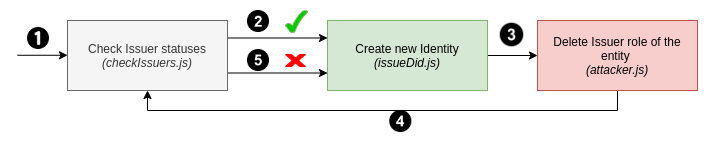
\includegraphics[width=1.1\textwidth]{images/PoC/poc-flow.png}
    \caption{Attack flow}
    \label{fig:poc-flow}
\end{figure}

The \acrshort{poc} consists of five parts. First, a script written in \textit{NodeJS} (listing \ref{lst:checkIssuers.js}) has been created, which checks whether the entity and the attacker have the role of Issuer. In the first step (1) it will check that the entity is an Issuer, but the attacker is not.\\
\lstinputlisting[label={lst:checkIssuers.js}, caption=checkIssuers.js source code, language=ES6]{examples/poc/checkIssuers.js}

Then it will be tested that the entity can correctly create new identities (2), for this we will use the script, also written in \textit{NodeJS} \textit{"issueDid.js"} (listing \ref{lst:issueDid.js}). After the execution, it will be possible to see the new \acrshort{did} created.\\
\lstinputlisting[label={lst:issueDid.js}, caption=issueDid.js source code, language=ES6]{examples/poc/issueDid.js}

The third step is the attack itself (3). At this point, the attacker (who we know is not an Issuer) will remove the entity from the Issuers list. Thus getting the entity to stop providing the service of creating identities, which can mean a lack of integrity and availability. This script is also written in \textit{NodeJS} (listing \ref{lst:attacker.js}).\\
\lstinputlisting[label={lst:attacker.js}, caption=attacker.js source code, language=ES6]{examples/poc/attacker.js}

Having carried out the attack successfully, only the last steps are missing, which basically is to repeat the first two to verify that the entity has stopped being able to provide the service. First we will check if the entity and the attacker are Issuers (4) but we will see that now neither of them has that role. This will be done by running the script \textit{checkIssuers.js} (listing \ref{lst:checkIssuers.js}) again. \\

Finally, we will try to create a new identity (5) with the \textit{issueDid.js} script, but we will not be able to generate a \acrshort{did} this time and checking the inability of the service.\\

To be able to re-establish the service in the entity, we would need a second entity with the role of Issuer, and that would add the first entity as Issuer. But even so, the same problem would still exist, and any malicious Subject (attacker) could carry out the attack again.
